\begin{figure}[H]
  \centering
  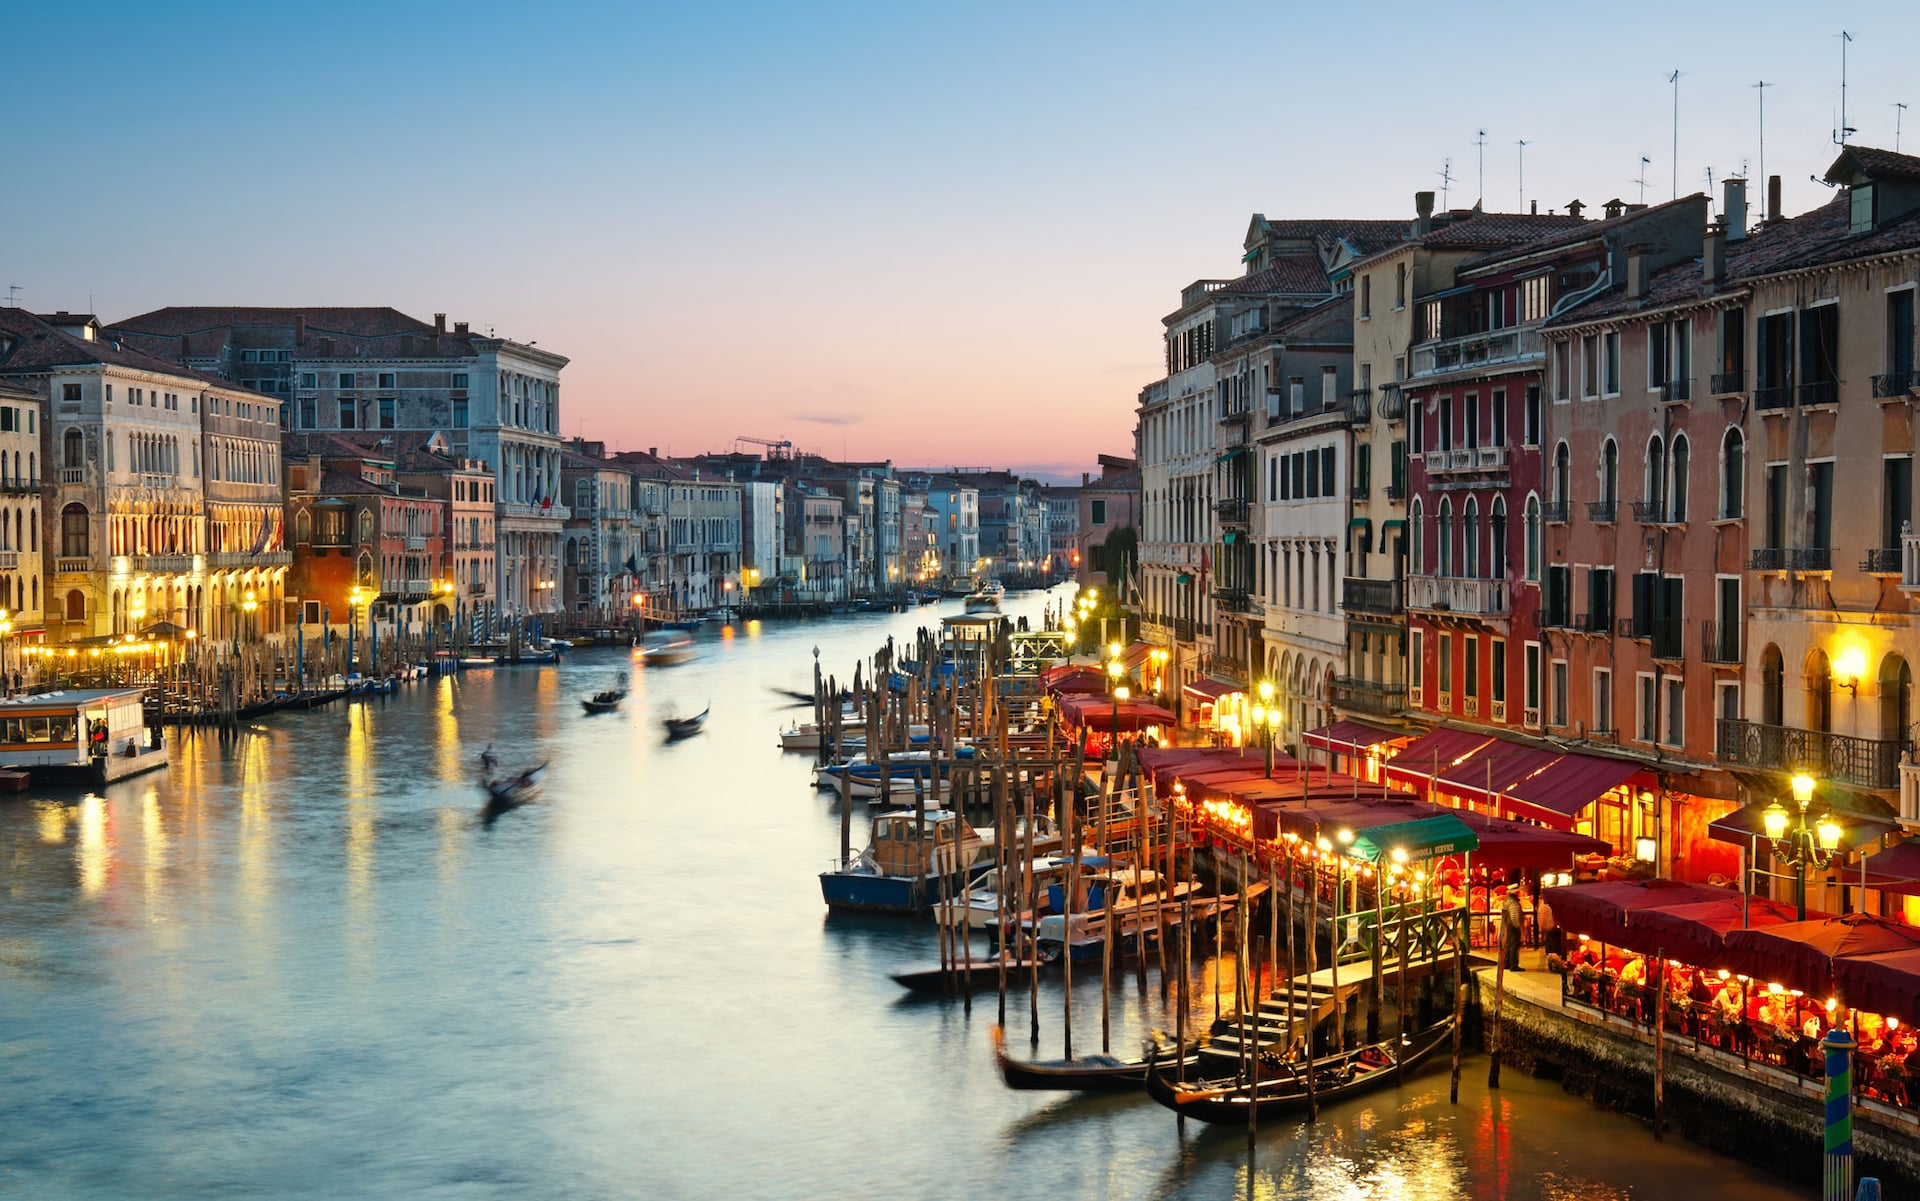
\includegraphics[width=\textwidth]{../../References/Images/Dynamia/venice-restaurants-by-canal}
  \caption{Reference image for Dynamia}
\end{figure}

\begin{figure}[H]
  \centering
  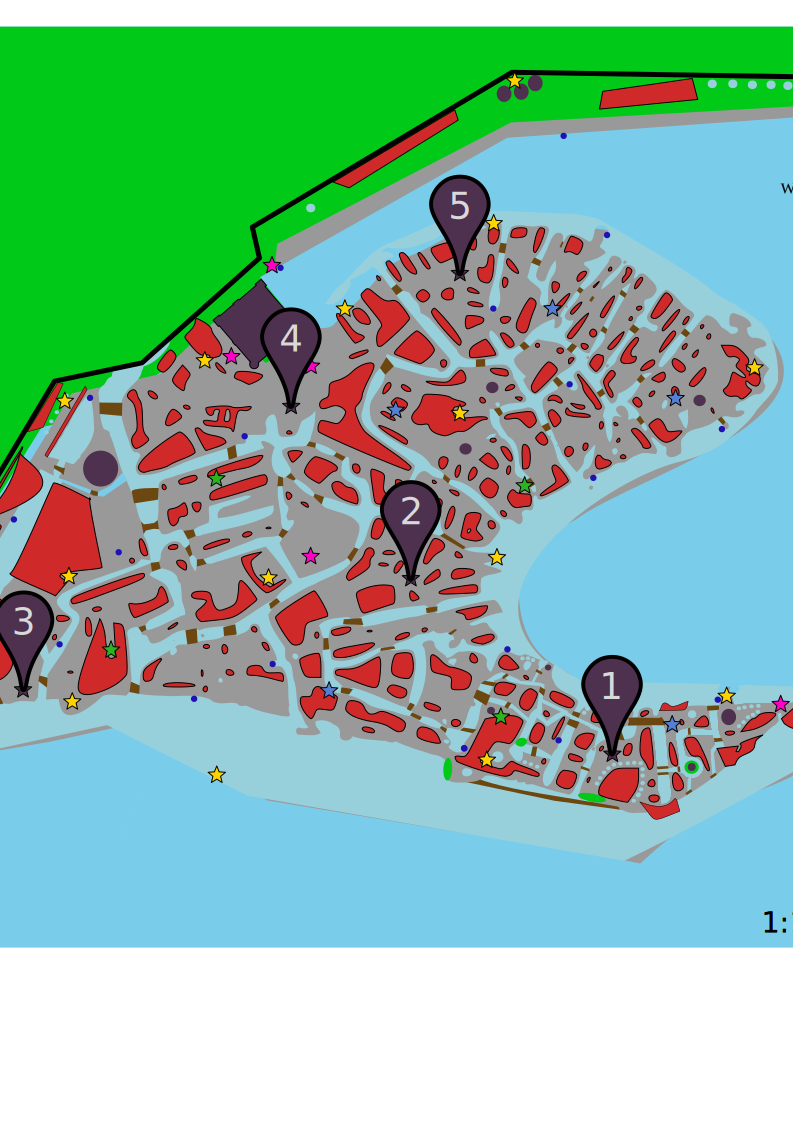
\includegraphics[width=\textwidth]{Images/Maps/dynamia}
  \caption{Map of Dynamia}
\end{figure}

The city is loosely based on Venice.

It is the capital of the Kingdom of Strangia. It is built on a lagoon and its streets are canals. Most of the quarters are placed on a small island connected to nearby ones by bridges.

It is a very beautiful and distinctive city, all the buildings are very colorful and there are many famous monuments. Thanks to its position, it is a very important business hub and there are merchants from many different countries. Despite the ongoing war, its market is very renowned and there you can find a lot of exotic products.

There are some guards and demons that patrol the city, but the atmosphere is quite peaceful. On direct orders of queen, each citizen has to do his best for the nation and any offender will be harshly punished.

There are some small shrubs that grow between the bricks of the building, quite big palms and vines on the walls. Some houses have beautiful and very manicured gardens, in particular in downtown.

On the streets there are some stray dogs and cats, mice and a lot of seagulls.

The city is divided in 4 macro areas and it has some characteristic landmarks that will be described here below.

For more reference images: \url{http://wastelandsteam.altervista.org/dynamia/}\\
Password: \textit{gld18}
